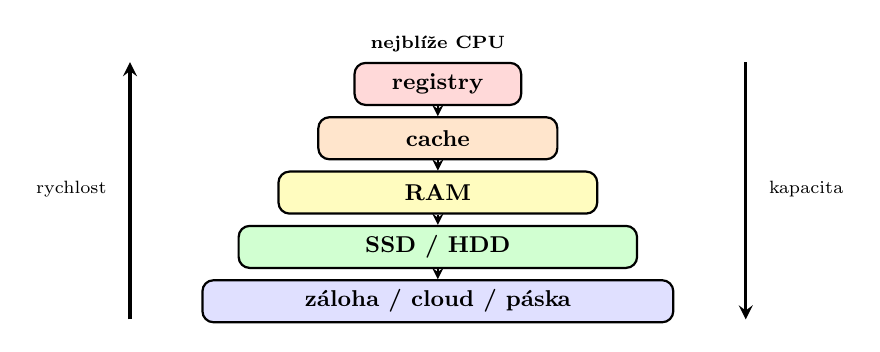
\begin{tikzpicture}[
    scale=0.92,
    transform shape,
    x=1cm, y=1cm,
    >=stealth,
    every node/.style={font=\small},
    level/.style={
        draw,
        thick,
        rounded corners,
        align=center,
        minimum height=0.58cm
    },
    arrowlabel/.style={
        font=\scriptsize,
        align=center
    }
]

    % Levels of hierarchy
    \node[
        level,
        fill=red!15,
        minimum width=2.3cm
    ] (reg) at (0,1.80) {\textbf{registry}};

    \node[
        level,
        fill=orange!20,
        minimum width=3.3cm
    ] (cache) at (0,1.05) {\textbf{cache}};

    \node[
        level,
        fill=yellow!25,
        minimum width=4.4cm
    ] (ram) at (0,0.30) {\textbf{RAM}};

    \node[
        level,
        fill=green!18,
        minimum width=5.5cm
    ] (ssd) at (0,-0.45) {\textbf{SSD / HDD}};

    \node[
        level,
        fill=blue!12,
        minimum width=6.5cm
    ] (archive) at (0,-1.20) {\textbf{záloha / cloud / páska}};

    % Vertical arrows between levels
    \draw[->, thick] (reg.south) -- (cache.north);
    \draw[->, thick] (cache.south) -- (ram.north);
    \draw[->, thick] (ram.south) -- (ssd.north);
    \draw[->, thick] (ssd.south) -- (archive.north);

    % Left side arrow - speed and price per bit increase upwards
    \draw[->, very thick] (-4.25,-1.45) -- (-4.25,2.10);
    \node[arrowlabel, anchor=east] at (-4.45,0.35)
        {rychlost};

    % Right side arrow - capacity increases downwards
    \draw[->, very thick] (4.25,2.10) -- (4.25,-1.45);
    \node[arrowlabel, anchor=west] at (4.45,0.35)
        {kapacita};

    % CPU label above
    \node[font=\scriptsize\bfseries] at (0,2.35) {nejblíže CPU};

\end{tikzpicture}
